\documentclass[12pt]{article} 

\usepackage[top=2.54cm, bottom=2.54cm, left=2.54cm, right=2.54cm]{geometry}
\usepackage{amsmath,amsthm,amsfonts,amssymb,enumerate}
\usepackage{graphicx}

\author{William Mairs and Katya Malison}
\title{Pies and Areas: a Comparison}
\begin{document}  
\maketitle

\pagestyle{empty}      %%% uncomment this to remove page numbers
% \pagestyle{plain}
We proposed two hypotheses:
\begin{enumerate}[-]
\item Single-color pie charts will result in higher accuracy than single-color area charts.
\item Single-color pie charts will result in higher accuracy than highlighted area charts.
\end{enumerate}
To test this participants were asked to report the percentage of a whole aera taken up by a section of an area chart and a slice of a pie chart. 
\begin{center}
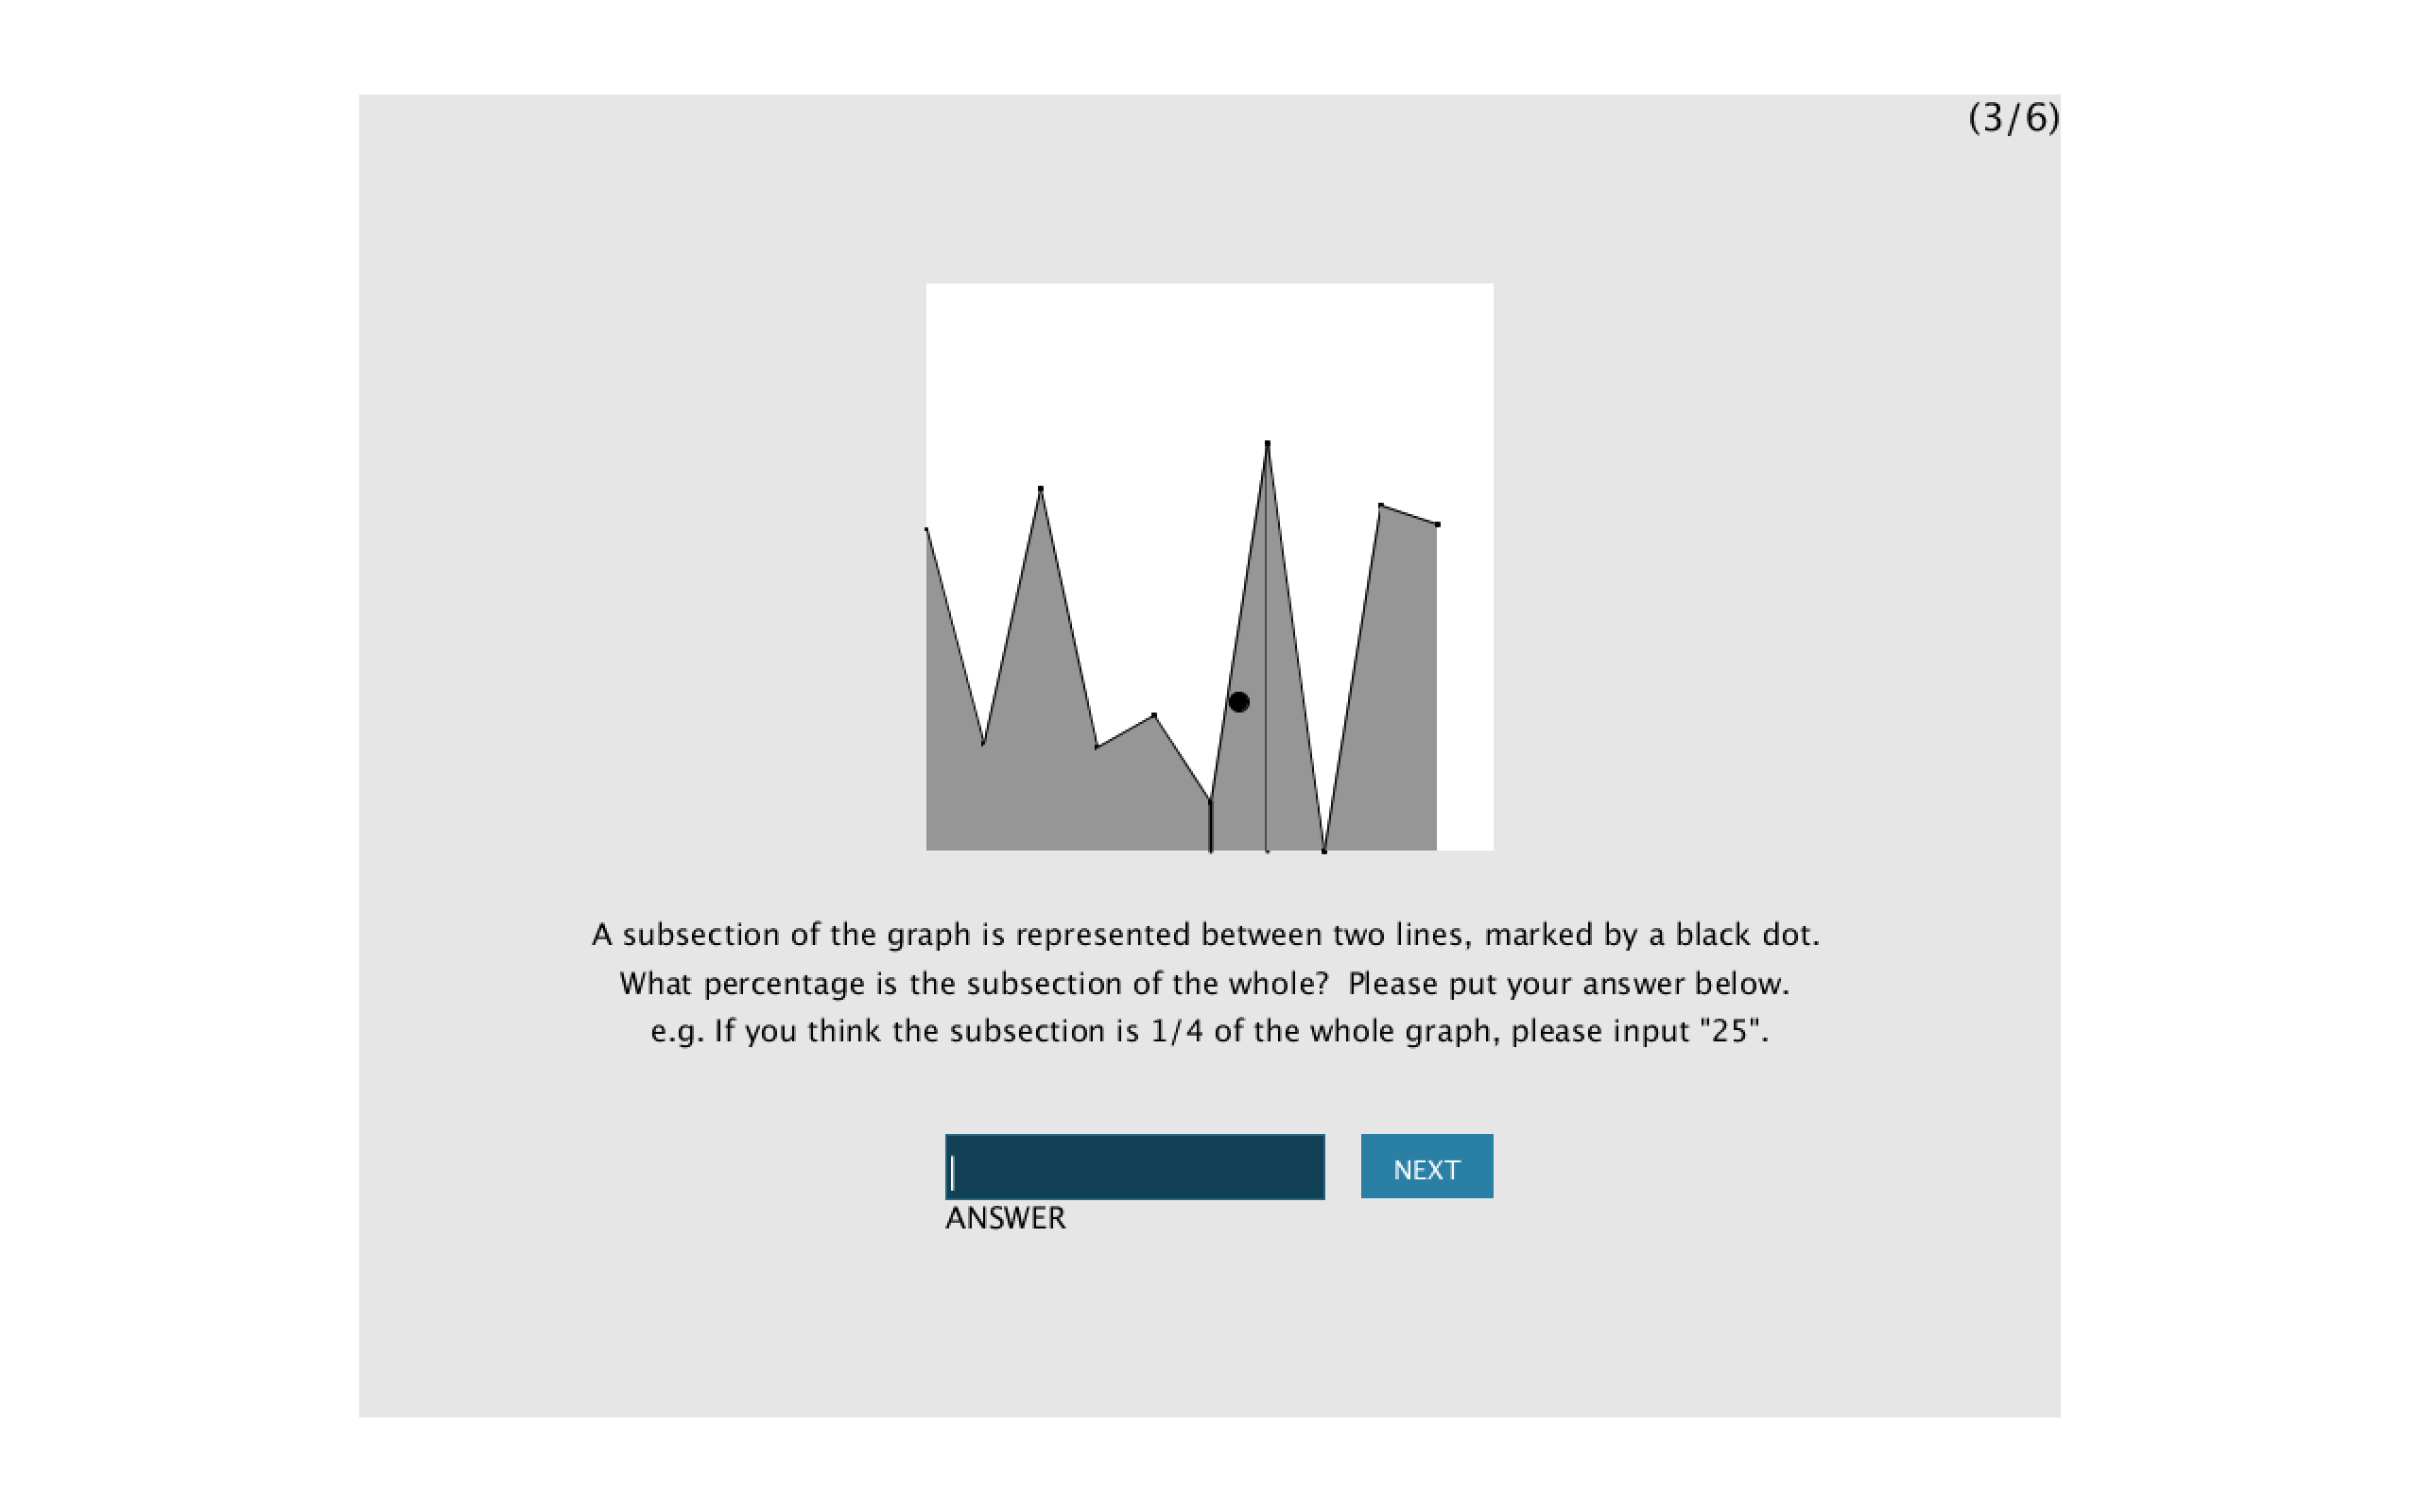
\includegraphics[width=5in]{monochrome_area.png}
\end{center}
Participants first reported on monochromatically colored charts.
\begin{center}
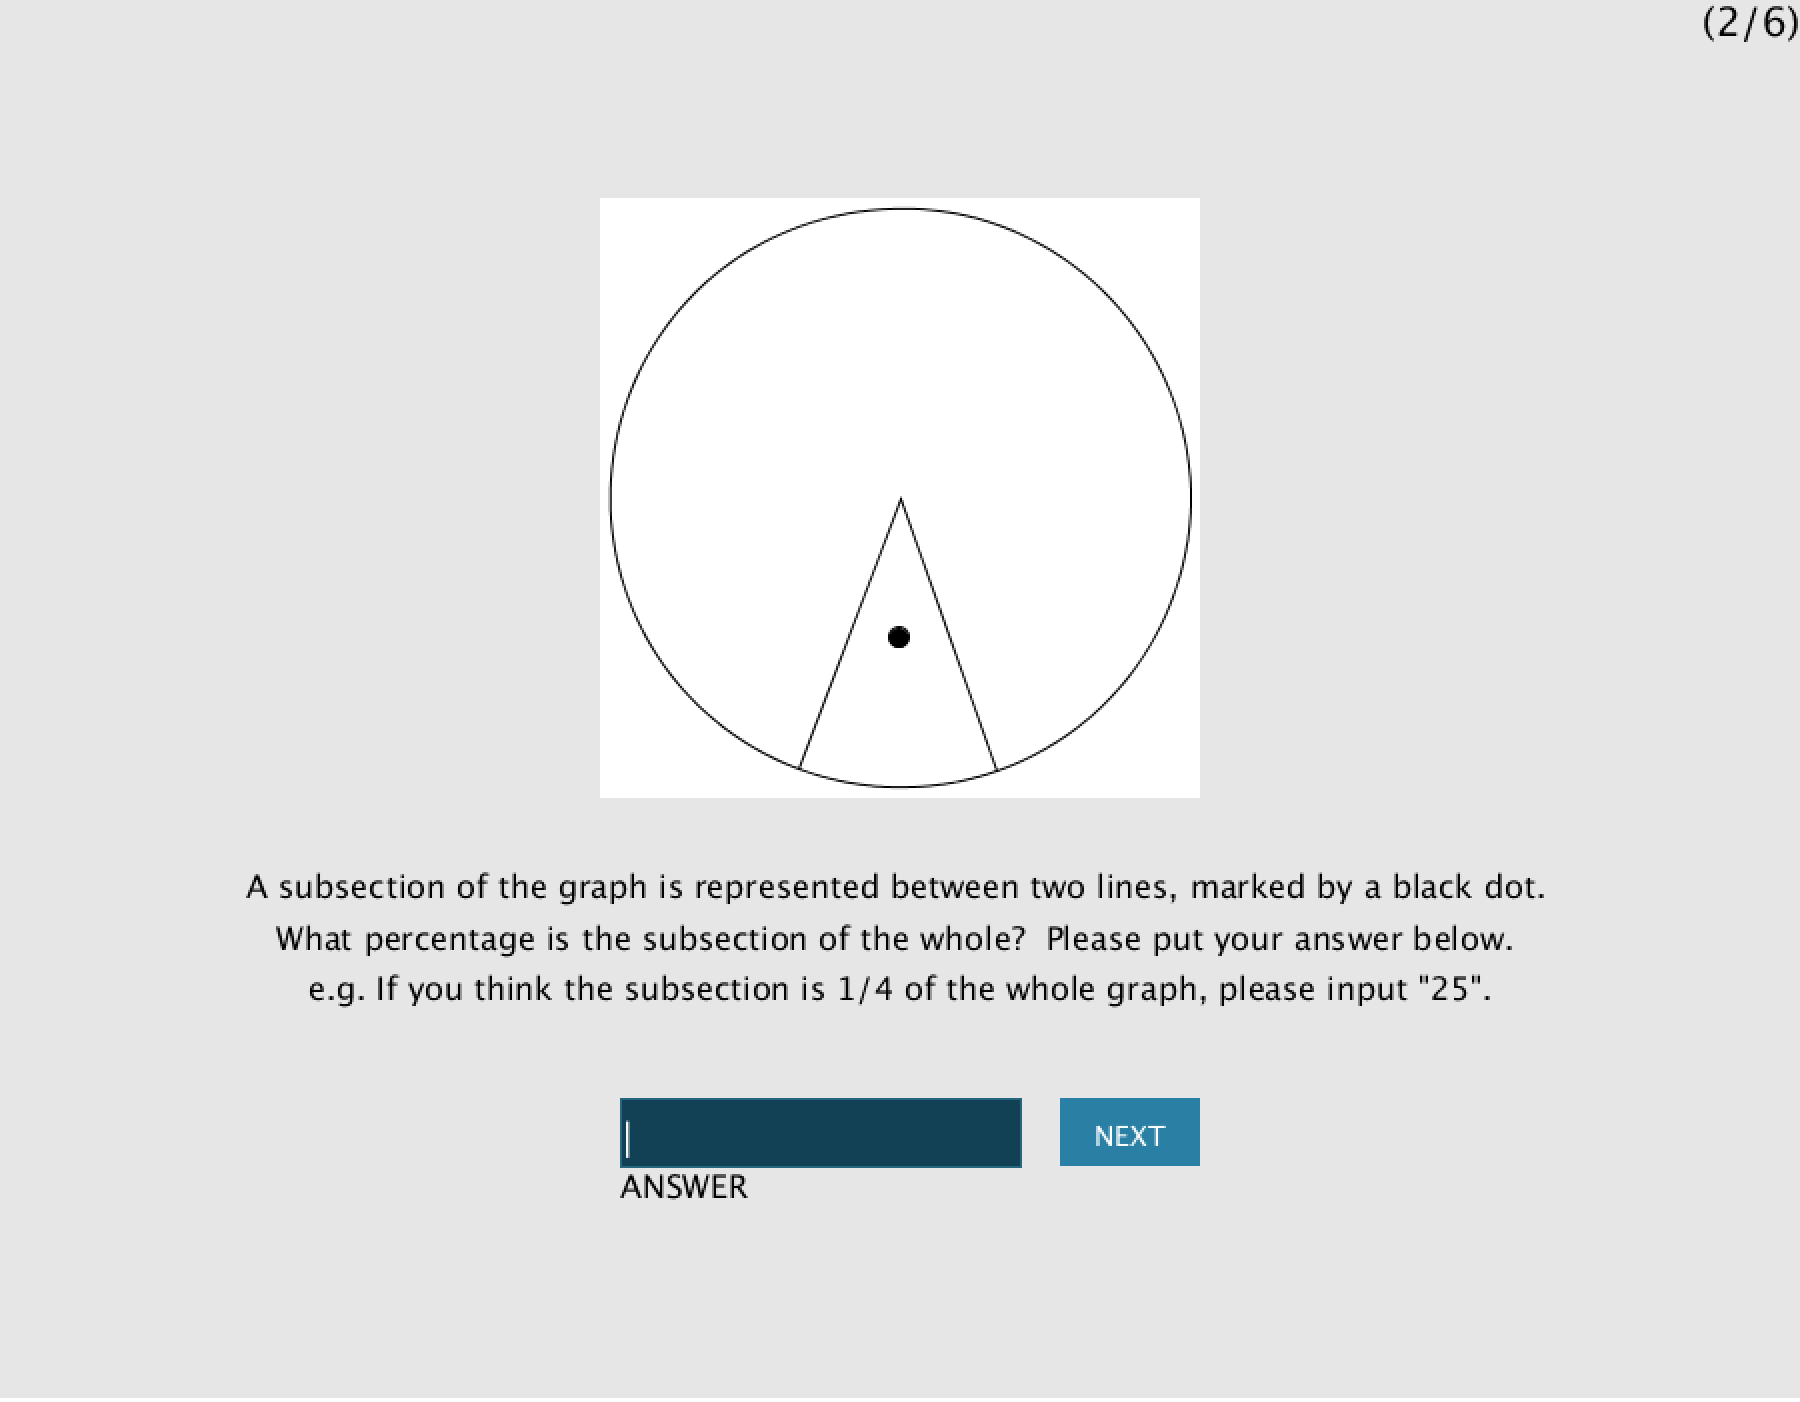
\includegraphics[width=5in]{monochrome_pie.png}
\end{center}
For the second part of the experiment, participants reported on area charts with one section highlighted.  During this part, the pie charts remained monochromatically colored.
\begin{center}
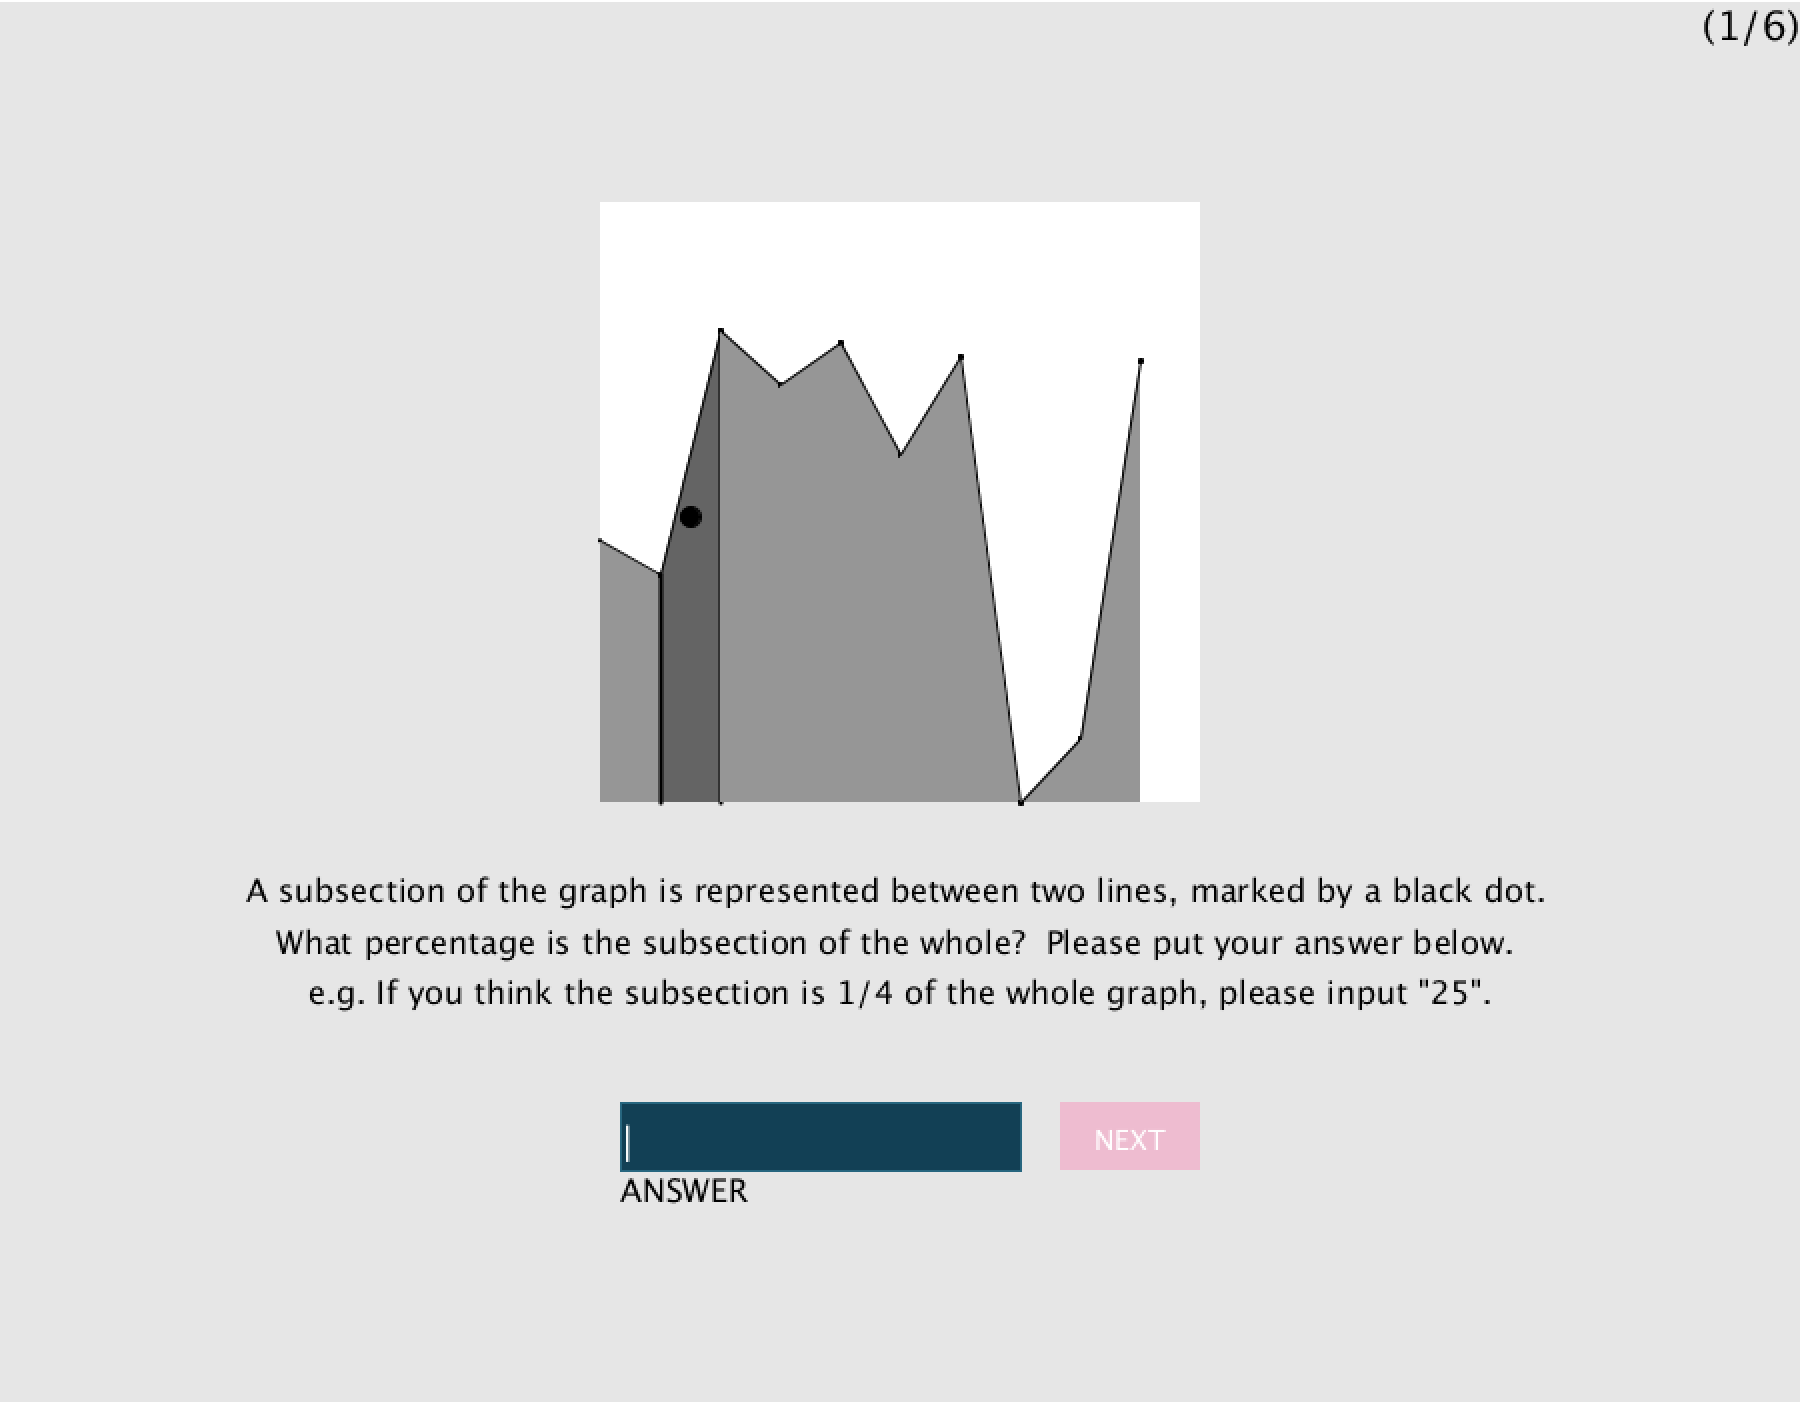
\includegraphics[width=5in]{shaded_area.png}
\end{center}
The experiment was conducted on eleven participants.  Each phase of the experiment included three of each kind of graph.  A visualization of the mean error and 95 percent confidence intervals for both charts in each phase is shown.  Confidence intervals were calculated using the R programming language, reading in .csv files, and using the quantile function for t distribution to calculate the error.
\begin{center}
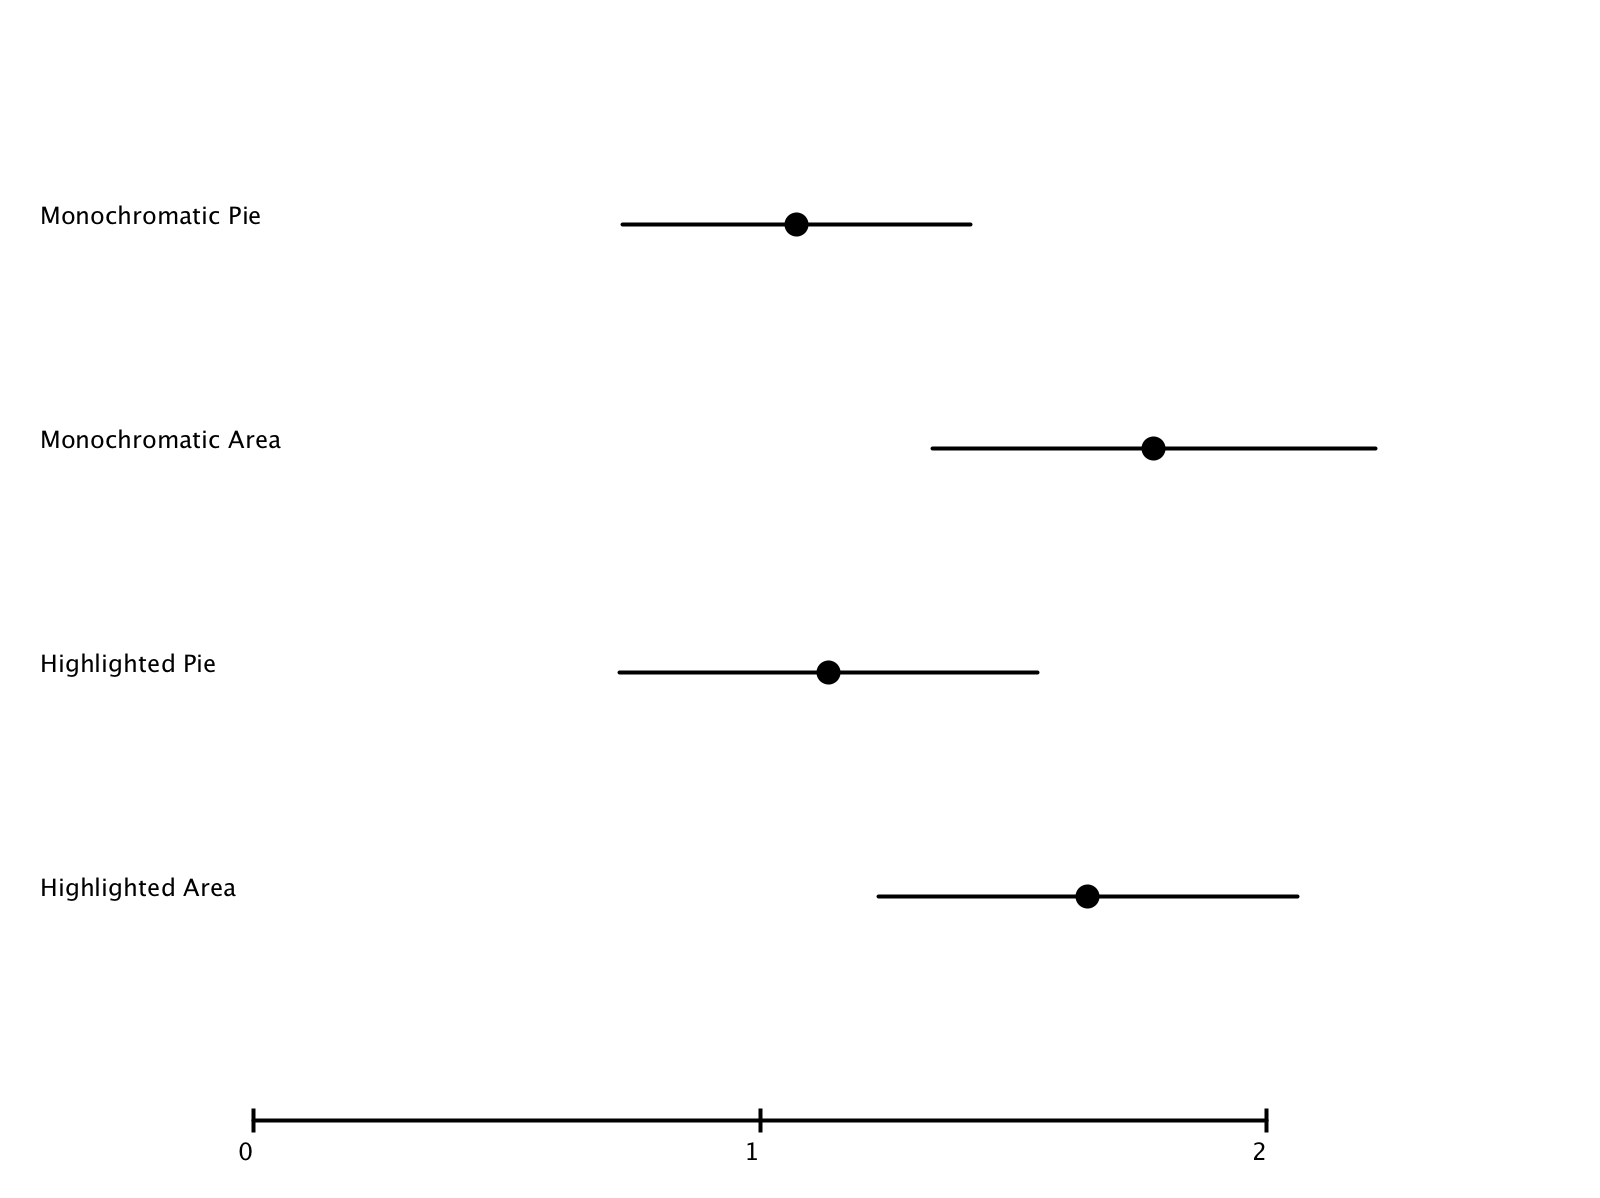
\includegraphics[width=5in]{confidence_intervals.png}
\end{center}
Our hypotheses are supported by this data.  Participants were less accurate reporting the percent areas of both monochromatic and highlighted area charts as compared to reporting percent areas of monochromatic pie charts.

\end{document}






















